\documentclass{article}
\usepackage[utf8]{inputenc}
\usepackage{tikz}
\title{Preimage Attack for Reduced Round keccak}
\date{June 2018}

\begin{document}

\maketitle

\section{Preimages on 2 Rounds of the 384-bit Hash function}

\begin{center}
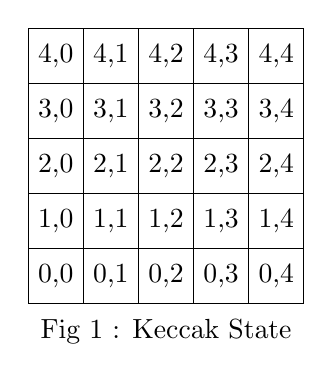
\begin{tikzpicture}[scale=.7]
\draw (0,0) grid (5,5);
    \node[] at (0.5,0.5) {0,0};
    \node[] at (1.5,0.5) {0,1};
    \node[] at (2.5,0.5) {0,2};
    \node[] at (3.5,0.5) {0,3};
    \node[] at (4.5,0.5) {0,4};

    \node[] at (0.5,1.5) {1,0};
    \node[] at (1.5,1.5) {1,1};
    \node[] at (2.5,1.5) {1,2};
    \node[] at (3.5,1.5) {1,3};
    \node[] at (4.5,1.5) {1,4};

    \node[] at (0.5,2.5) {2,0};
    \node[] at (1.5,2.5) {2,1};
    \node[] at (2.5,2.5) {2,2};
    \node[] at (3.5,2.5) {2,3};
    \node[] at (4.5,2.5) {2,4};

    \node[] at (0.5,3.5) {3,0};
    \node[] at (1.5,3.5) {3,1};
    \node[] at (2.5,3.5) {3,2};
    \node[] at (3.5,3.5) {3,3};
    \node[] at (4.5,3.5) {3,4};

    \node[] at (0.5,4.5) {4,0};
    \node[] at (1.5,4.5) {4,1};
    \node[] at (2.5,4.5) {4,2};
    \node[] at (3.5,4.5) {4,3};
    \node[] at (4.5,4.5) {4,4};
    
    \node[anchor=center] at (2.5, -0.5) {Fig 1 : Keccak State};
\end{tikzpicture}
\end{center}

In this section we present a preimage attack for a reduced version with two rounds of Keccak. The preimage can be found in $2^{88}$ time and $2^{87}$ memory. It is not practical, but is an improvement from the present 2 round preimage attack for Keccak-384 which takes $2^{129}$ time [1].

\subsection{Main Scheme}
The Preimage attack on 2 rounds is represented in figure 2.\newline

In Fig 2, each slice represents different states. For the sake of simplicity, we will omit the $\iota$ transformation in the explanation, as it doesnt affect the procedure of the attack, but should be taken into account when implementing the attack (though not practical).

\newpar
We are given a hash value which is 6 lanes in State 4[Fig 2], which represents the output of Keccak permutation. We need to find a messafe block that produces the same hash value. In Fig2 State 1 the lanes marked with (a0, a1, a2, b0, b1, b2, c0, c1, c2, d0, d1, e0, e1) are the parts of the message that we dont fix until the end of the attack.
The conditions are that : $a2 = a0 \oplus a1$,  $b2 = b0 \oplus b1$, $c2 = c0 \oplus c1$, $d0 = d1 = 0$, $e0 = e1$. Due to these conditions the first $\theta$ operation doesn't affect the state 1 [Fig 2.] From the initial state 1 we can then compute the known lanes in state 2 after $\theta, \rho$ and $\pi$, as well as the positions of the unknown lanes.
\newpar
The change of state from state 1 to state 2 shows the movement of lanes in detail, the number shown in round brackets along with the variable in state 2 is due to $\rho$. Imposing the previous conditions we still have 7*64 degrees of freedom for the message, which is greater than the number of bits of the hash output i.e. 6*64, so we can expect to find atleast one solution.\newline

\begin{center}
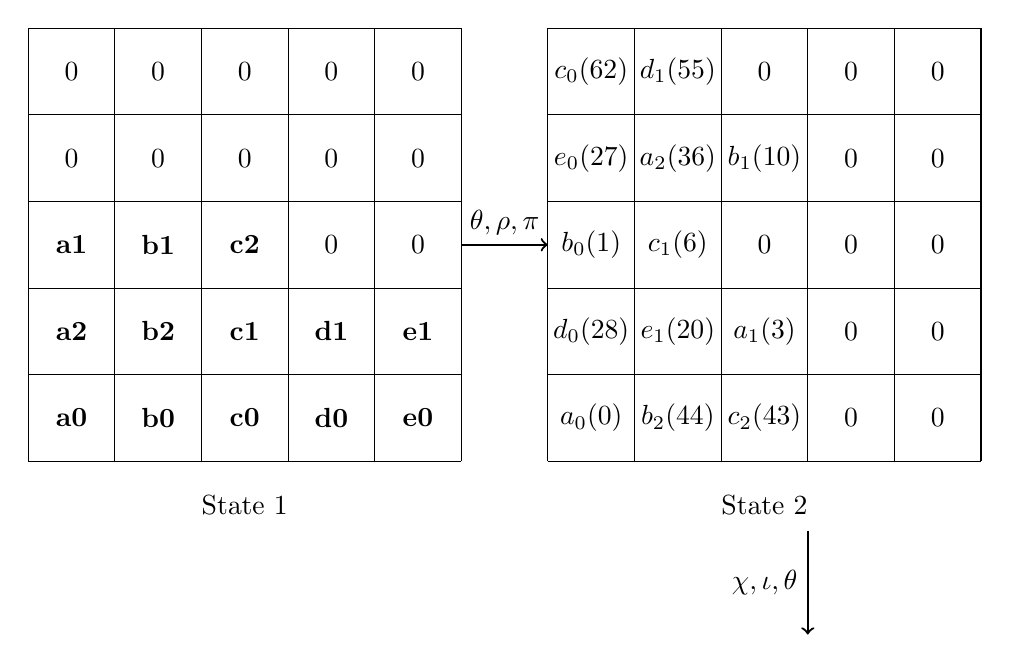
\begin{tikzpicture}[scale=1.1]
\draw (0,0) grid (5,5);
    \node[] at (0.5,0.5) {\textbf{a0}};
    \node[] at (1.5,0.5) {\textbf{b0}};
    \node[] at (2.5,0.5) {\textbf{c0}};
    \node[] at (3.5,0.5) {\textbf{d0}};
    \node[] at (4.5,0.5) {\textbf{e0}};

    \node[] at (0.5,1.5) {\textbf{a2}};
    \node[] at (1.5,1.5) {\textbf{b2}};
    \node[] at (2.5,1.5) {\textbf{c1}};
    \node[] at (3.5,1.5) {\textbf{d1}};
    \node[] at (4.5,1.5) {\textbf{e1}};

    \node[] at (0.5,2.5) {\textbf{a1}};
    \node[] at (1.5,2.5) {\textbf{b1}};
    \node[] at (2.5,2.5) {\textbf{c2}};
    \node[] at (3.5,2.5) {0};
    \node[] at (4.5,2.5) {0};

    \node[] at (0.5,3.5) {0};
    \node[] at (1.5,3.5) {0};
    \node[] at (2.5,3.5) {0};
    \node[] at (3.5,3.5) {0};
    \node[] at (4.5,3.5) {0};

    \node[] at (0.5,4.5) {0};
    \node[] at (1.5,4.5) {0};
    \node[] at (2.5,4.5) {0};
    \node[] at (3.5,4.5) {0};
    \node[] at (4.5,4.5) {0};

\node[anchor=center] at (2.5, -0.5) {State 1};

\draw (6,0) grid (11,5);
    \node[] at (6.5,0.5) {$a_0$(0)};
    \node[] at (7.5,0.5) {$b_2$(44)};
    \node[] at (8.5,0.5) {$c_2$(43)};
    \node[] at (9.5,0.5) {0};
    \node[] at (10.5,0.5) {0};

    \node[] at (6.5,1.5) {$d_0$(28)};
    \node[] at (7.5,1.5) {$e_1$(20)};
    \node[] at (8.5,1.5) {$a_1$(3)};
    \node[] at (9.5,1.5) {0};
    \node[] at (10.5,1.5) {0};

    \node[] at (6.5,2.5) {$b_0$(1)};
    \node[] at (7.5,2.5) {$c_1$(6)};
    \node[] at (8.5,2.5) {0};
    \node[] at (9.5,2.5) {0};
    \node[] at (10.5,2.5) {0};

    \node[] at (6.5,3.5) {$e_0$(27)};
    \node[] at (7.5,3.5) {$a_2$(36)};
    \node[] at (8.5,3.5) {$b_1$(10)};
    \node[] at (9.5,3.5) {0};
    \node[] at (10.5,3.5) {0};

    \node[] at (6.5,4.5) {$c_0$(62)};
    \node[] at (7.5,4.5) {$d_1$(55)};
    \node[] at (8.5,4.5) {0};
    \node[] at (9.5,4.5) {0};
    \node[] at (10.5,4.5) {0};

\node[anchor=center] at (8.5, -0.5) {State 2};
    \draw[thick,->] (5, 2.5) -- node [above] {$\theta, \rho, \pi$} (6,2.5);
    \draw[thick,->] (9, -0.8) -- node [left] {$\chi, \iota, \theta$} (9, -2);
\end{tikzpicture}
\end{center}
% \[
% \]
\begin{center}
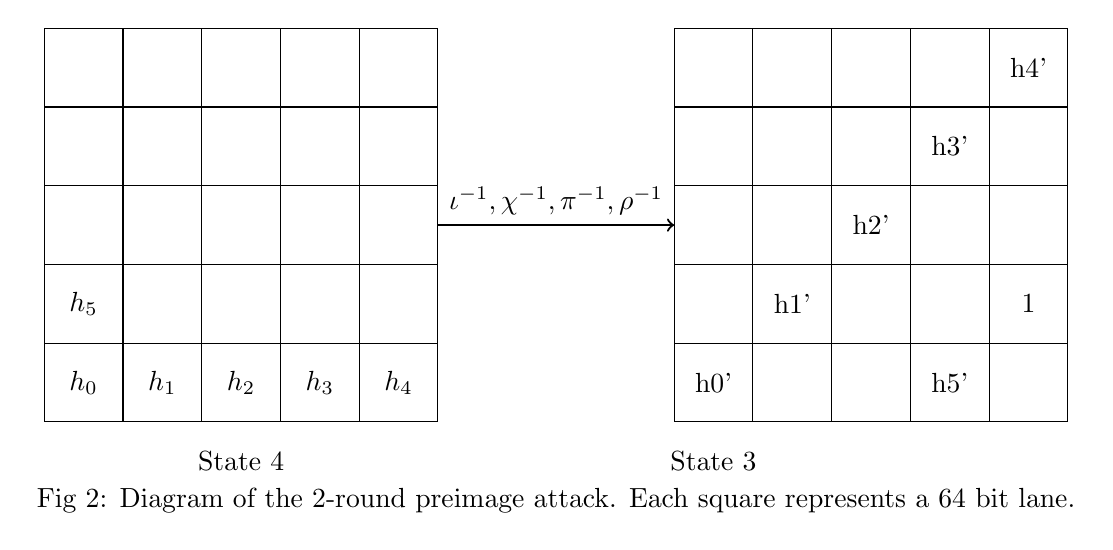
\begin{tikzpicture}[scale=1]
\draw (2,0) grid (7,5);
    \node[] at (2.5,0.5) {$h_0$};
    \node[] at (3.5,0.5) {$h_1$};
    \node[] at (4.5,0.5) {$h_2$};
    \node[] at (5.5,0.5) {$h_3$};
    \node[] at (6.5,0.5) {$h_4$};

    \node[] at (2.5,1.5) {$h_5$};
    \node[] at (3.5,1.5) { };
    \node[] at (4.5,1.5) { };
    \node[] at (5.5,1.5) { };
    \node[] at (6.5,1.5) { };

    \node[] at (2.5,2.5) { };
    \node[] at (3.5,2.5) { };
    \node[] at (4.5,2.5) { };
    \node[] at (5.5,2.5) { };
    \node[] at (6.5,2.5) { };

    \node[] at (2.5,3.5) { };
    \node[] at (3.5,3.5) { };
    \node[] at (4.5,3.5) { };
    \node[] at (5.5,3.5) { };
    \node[] at (6.5,3.5) { };

    \node[] at (2.5,4.5) { };
    \node[] at (3.5,4.5) { };
    \node[] at (4.5,4.5) { };
    \node[] at (5.5,4.5) { };
    \node[] at (6.5,4.5) { };

\draw (10,0) grid (15,5);
    \node[] at (10.5,0.5) {h0'};
    \node[] at (11.5,0.5) { };
    \node[] at (12.5,0.5) { };
    \node[] at (13.5,0.5) {h5'};
    \node[] at (14.5,0.5) { };

    \node[] at (10.5,1.5) { };
    \node[] at (11.5,1.5) {h1'};
    \node[] at (12.5,1.5) { };
    \node[] at (13.5,1.5) { };
    \node[] at (14.5,1.5) {1};

    \node[] at (10.5,2.5) { };
    \node[] at (11.5,2.5) { };
    \node[] at (12.5,2.5) {h2'};
    \node[] at (13.5,2.5) { };
    \node[] at (14.5,2.5) { };

    \node[] at (10.5,3.5) { };
    \node[] at (11.5,3.5) { };
    \node[] at (12.5,3.5) { };
    \node[] at (13.5,3.5) {h3'};
    \node[] at (14.5,3.5) { };

    \node[] at (10.5,4.5) { };
    \node[] at (11.5,4.5) { };
    \node[] at (12.5,4.5) { };
    \node[] at (13.5,4.5) { };
    \node[] at (14.5,4.5) {h4'};
    
    \node[anchor=center] at (10.5, -0.5) {State 3};
    \node[anchor=center] at (4.5, -0.5) {State 4};
     \draw[thick,->] (7, 2.5) -- node [above] {$\iota^{-1}, \chi^{-1}, \pi^{-1}, \rho^{-1}$} (10,2.5);
     \node[anchor=center] at (8.5, -1) {Fig 2: Diagram of the 2-round preimage attack. Each square represents a 64 bit lane.};
\end{tikzpicture}
\end{center}    
\newpage
\newpar
In the backward direction, we can invert from State 4, the known 6 lanes in final state with $\chi^{-1}$. The first five lanes can be directly inverted using $\chi^{-1}$, for the remaining sixth lane, we can fix the seventh lane of State 5 to \textbf{1} for inverting sixth lane. As shown in Fig 3. Then, we can apply the inverse of $\pi$ and of $\rho$ and obtain the values and positions of the 6 known lanes in State 3.

\begin{center}
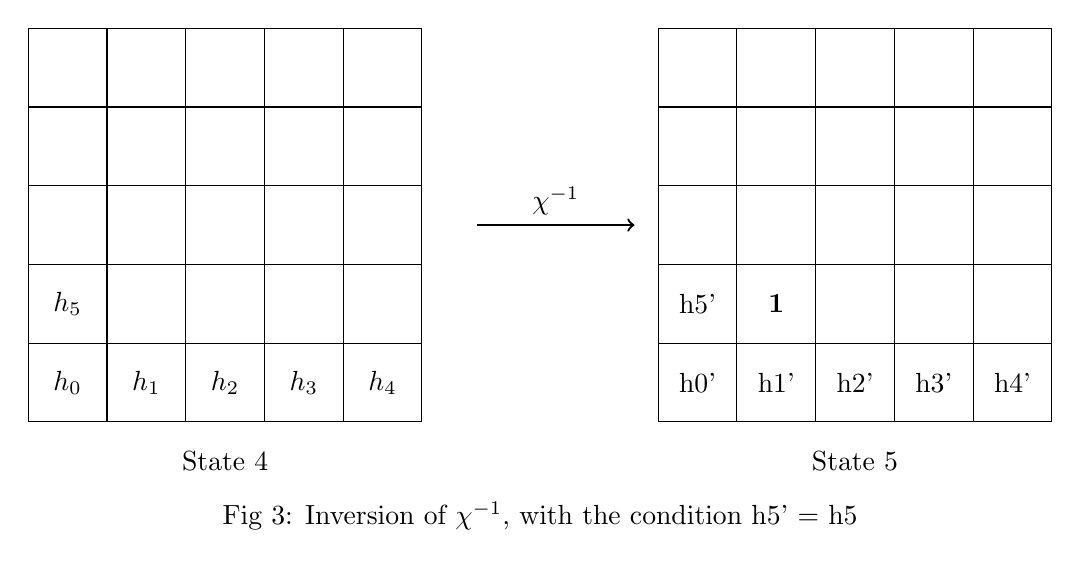
\begin{tikzpicture}[scale=1]
\draw (2,0) grid (7,5);
    \node[] at (2.5,0.5) {$h_0$};
    \node[] at (3.5,0.5) {$h_1$};
    \node[] at (4.5,0.5) {$h_2$};
    \node[] at (5.5,0.5) {$h_3$};
    \node[] at (6.5,0.5) {$h_4$};

    \node[] at (2.5,1.5) {$h_5$};
    \node[] at (3.5,1.5) { };
    \node[] at (4.5,1.5) { };
    \node[] at (5.5,1.5) { };
    \node[] at (6.5,1.5) { };

    \node[] at (2.5,2.5) { };
    \node[] at (3.5,2.5) { };
    \node[] at (4.5,2.5) { };
    \node[] at (5.5,2.5) { };
    \node[] at (6.5,2.5) { };

    \node[] at (2.5,3.5) { };
    \node[] at (3.5,3.5) { };
    \node[] at (4.5,3.5) { };
    \node[] at (5.5,3.5) { };
    \node[] at (6.5,3.5) { };

    \node[] at (2.5,4.5) { };
    \node[] at (3.5,4.5) { };
    \node[] at (4.5,4.5) { };
    \node[] at (5.5,4.5) { };
    \node[] at (6.5,4.5) { };

\draw (10,0) grid (15,5);
    \node[] at (10.5,0.5) {h0'};
    \node[] at (11.5,0.5) {h1'};
    \node[] at (12.5,0.5) {h2'};
    \node[] at (13.5,0.5) {h3'};
    \node[] at (14.5,0.5) {h4'};

    \node[] at (10.5,1.5) {h5'};
    \node[] at (11.5,1.5) {\textbf{1}};
    \node[] at (12.5,1.5) { };
    \node[] at (13.5,1.5) { };
    \node[] at (14.5,1.5) { };

    \node[] at (10.5,2.5) { };
    \node[] at (11.5,2.5) { };
    \node[] at (12.5,2.5) { };
    \node[] at (13.5,2.5) { };
    \node[] at (14.5,2.5) { };

    \node[] at (10.5,3.5) { };
    \node[] at (11.5,3.5) { };
    \node[] at (12.5,3.5) { };
    \node[] at (13.5,3.5) { };
    \node[] at (14.5,3.5) { };

    \node[] at (10.5,4.5) { };
    \node[] at (11.5,4.5) { };
    \node[] at (12.5,4.5) { };
    \node[] at (13.5,4.5) { };
    \node[] at (14.5,4.5) { };
    
    \node[anchor=center] at (12.5, -0.5) {State 5};
    \node[anchor=center] at (4.5, -0.5) {State 4};
     \draw[thick,->] (7.7, 2.5) -- node [above] {$\chi^{-1}$} (9.7,2.5);
     \node[anchor=center] at (8.5, -1.2) {Fig 3: Inversion of $\chi^{-1}$, with the condition h5' = h5};
\end{tikzpicture}
\end{center}    

\newpar
Then, the issue is to find the values of the eleven 64-bit words (a0, a1, a2, b0, b1, b2, c0, c1, c2, e0, e1) in state 2 that make possible the transition by the operations $\chi$ and $\theta$ from the state 2, that we have obtained computing forward, to the state 3, that we have obtained computing backward. For this we start by finding the bits that verify the relations for few slices.  The idea is same as in [2]. The idea is, to consider first groups of 3 slices where we guess all the involved bits of a0,...,e1 and next we can do a sieving by just keeping the guesses ones that produce by $\chi$ and $\theta$ the values of the 7x2 = 14 known bits from State 3 in the middle and last slices of the group of three slices.This is possible as for computing the output of $\theta$ in a specific slice, we need to know this same slice and the previous one in the input state.

\subsection{Finding Partial Solutions}


\section{References :}

1. Jian Guo and Meicheng Liu and Ling Song, Linear Structures: Applications to Cryptanalysis of Round-Reduced Keccak.\newline
 

\end{document}
